\setproblem{1939}

\begin{frame}[label=p1]{중량제한(1939)}

\footnotesize

\begin{block}{문제}
$N(2 \le N \le 10{,}000)$개의 섬으로 이루어진 나라가 있다. 이들 중 몇 개의 섬 사이에는 다리가 설치되어 있어서 차들이 다닐 수 있다.

영식 중공업에서는 두 개의 섬에 공장을 세워 두고 물품을 생산하는 일을 하고 있다. 물품을 생산하다 보면 공장에서 다른 공장으로 생산 중이던 물품을 수송해야 할 일이 생기곤 한다. 그런데 각각의 다리마다 중량제한이 있기 때문에 무턱대고 물품을 옮길 수 없다. 만약 중량제한을 초과하는 양의 물품이 다리를 지나게 되면 다리가 무너지게 된다.

한 번의 이동에서 옮길 수 있는 물품들의 중량의 최댓값을 구하는 프로그램을 작성하시오.
\end{block}

\begin{block}{입력}
첫째 줄에 $N$, $M(1 \le M \le 100{,}000)$이 주어진다. 다음 $M$개의 줄에는 다리에 대한 정보를 나타내는 세 정수 $A$, $B(1 \le A, B \le N)$, $C(1 \le C \le 1{,}000{,}000{,}000)$가 주어진다. 이는 $A$번 섬과 $B$번 섬 사이에 중량제한이 $C$인 다리가 존재한다는 의미이다.

서로 같은 두 섬 사이에 여러 개의 다리가 있을 수도 있으며, 모든 다리는 양방향이다. 마지막 줄에는 공장이 위치해 있는 섬의 번호를 나타내는 서로 다른 두 정수가 주어진다. 공장이 있는 두 섬을 연결하는 경로는 항상 존재하는 데이터만 입력으로 주어진다.
\end{block}

\end{frame}

\begin{frame}{예시 그래프 $G$}

\footnotesize

\begin{center}
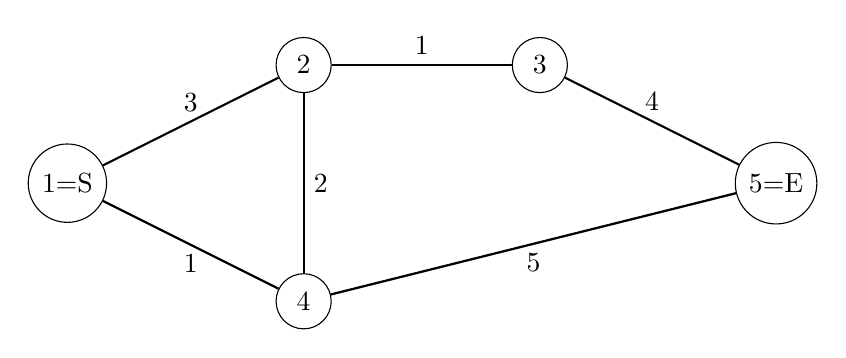
\begin{tikzpicture}[
    vertex/.style={circle, draw, minimum size=7mm},
    edge/.style={thick}
]

\node[vertex] (1) at (0,0) {1=S};
\node[vertex] (2) at (3,1.5) {2};
\node[vertex] (4) at (3,-1.5) {4};
\node[vertex] (3) at (6,1.5) {3};
\node[vertex] (5) at (9,0) {5=E};

\draw[edge] (1) -- node[above] {3} (2);
\draw[edge] (1) -- node[below] {1} (4);
\draw[edge] (2) -- node[above] {1} (3);
\draw[edge] (2) -- node[right] {2} (4);
\draw[edge] (3) -- node[above] {4} (5);
\draw[edge] (4) -- node[below] {5} (5);

\end{tikzpicture}
\end{center}

\end{frame}

\begin{frame}{데이크스트라 풀이}

\footnotesize
일반적인 가중치 있는 그래프에서 경로의 가중치는 간선들의 가중치의 합입니다. 즉 $w_1 + w_2 + \cdots + w_k$입니다. \\

이 문제에서는 가장 작은 간선의 가중치가 경로의 가중치입니다. 즉 $\min(w_1, w_2, \ldots, w_k)$입니다.
따라서, 경로의 길이를 구하는 방법을 $\min$ 연산으로 바꿔서 데이크스트라 알고리즘을 적용할 수 있습니다.

\end{frame}

\begin{frame}[fragile, allowframebreaks]{정의찬 데이크스트라 소스 코드}
\inputminted{java}{../src/\prob/uichan/Dijkstra.java}
\end{frame}

\begin{frame}[fragile, allowframebreaks]{서민종 데이크스트라 1 소스 코드}
\inputminted{java}{../src/\prob/minjong/Main.java}
\end{frame}

\begin{frame}[fragile, allowframebreaks]{서민종 데이크스트라 2 소스 코드}
\inputminted{java}{../src/\prob/minjong/Main2.java}
\end{frame}

\begin{frame}[fragile, allowframebreaks]{김준형 데이크스트라 소스 코드}
\inputminted{java}{../src/\prob/junhyeong/Main.java}
\end{frame}

\begin{frame}[fragile, allowframebreaks]{김지훈 데이크스트라 소스 코드}
\inputminted{java}{../src/\prob/jihoon/BOJ_1939.java}
\end{frame}

\begin{frame}[fragile, allowframebreaks]{임건애 데이크스트라 소스 코드}
\inputminted{java}{../src/\prob/keonae/Main.java}
\end{frame}

\begin{frame}[fragile, allowframebreaks]{김시온 데이크스트라 소스 코드}
\inputminted{java}{../src/\prob/sion/Dijkstra.java}
\end{frame}

\begin{frame}{부분 그래프 $G_w$}

\footnotesize

\begin{block}{정의}
$G_w$는 그래프 $G$의 모든 정점과 \textbf{가중치가 $w$ 이상인 간선만} 포함하는 그래프입니다.
\end{block}

\begin{center}
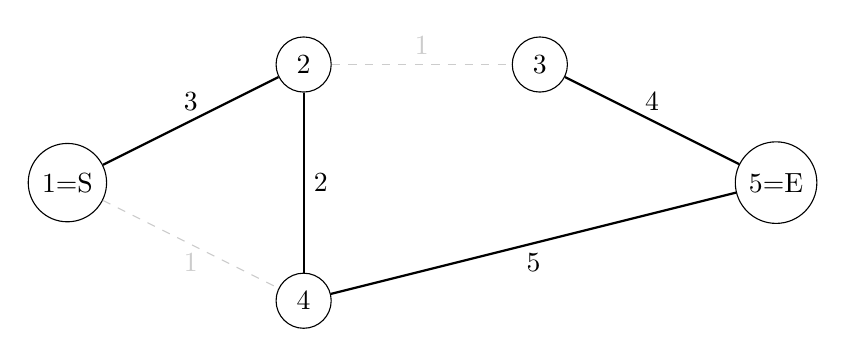
\begin{tikzpicture}[
    vertex/.style={circle, draw, minimum size=7mm},
    edge/.style={thick},
    removed/.style={gray!40,dashed}
]

\node[vertex] (1) at (0,0) {1=S};
\node[vertex] (2) at (3,1.5) {2};
\node[vertex] (4) at (3,-1.5) {4};
\node[vertex] (3) at (6,1.5) {3};
\node[vertex] (5) at (9,0) {5=E};

\draw[edge] (1) -- node[above] {3} (2);
\draw[removed] (1) -- node[below] {1} (4);
\draw[removed] (2) -- node[above] {1} (3);
\draw[edge] (2) -- node[right] {2} (4);
\draw[edge] (3) -- node[above] {4} (5);
\draw[edge] (4) -- node[below] {5} (5);

\end{tikzpicture}
\end{center}

예를 들어 위 그래프에서 $G_2$는 가중치가 $2$ 이상인 간선만 남긴 그래프입니다.

\end{frame}

\begin{frame}{$G_3$ 예시}

\footnotesize

\begin{center}
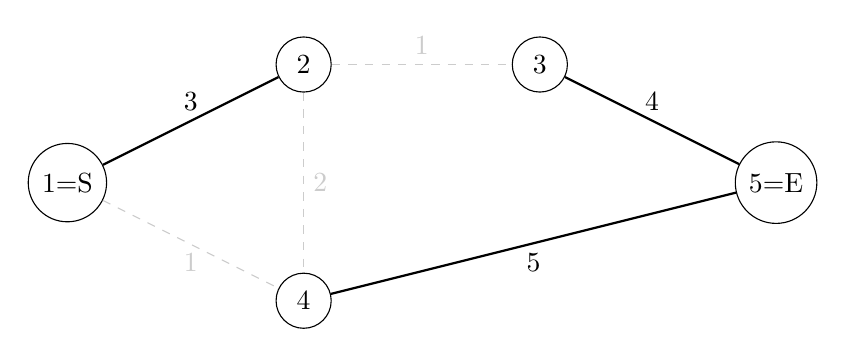
\begin{tikzpicture}[
    vertex/.style={circle, draw, minimum size=7mm},
    edge/.style={thick},
    removed/.style={gray!40,dashed}
]

\node[vertex] (1) at (0,0) {1=S};
\node[vertex] (2) at (3,1.5) {2};
\node[vertex] (4) at (3,-1.5) {4};
\node[vertex] (3) at (6,1.5) {3};
\node[vertex] (5) at (9,0) {5=E};

\draw[edge] (1) -- node[above] {3} (2);
\draw[removed] (1) -- node[below] {1} (4);
\draw[removed] (2) -- node[above] {1} (3);
\draw[removed] (2) -- node[right] {2} (4);
\draw[edge] (3) -- node[above] {4} (5);
\draw[edge] (4) -- node[below] {5} (5);

\end{tikzpicture}
\end{center}

$G_3$에서는 가중치가 $3$ 이상인 간선만 남습니다.

\end{frame}

\begin{frame}{$G_w$의 의미와 단조성}

\footnotesize

만약 $G_w$에서 $S$에서 $E$까지 경로가 존재한다면, \textbf{중량 $w$의 물품을 옮길 수 있습니다.}

\begin{block}{판정 문제}
$G_w$에서 $S$에서 $E$까지 경로가 존재하는가?
\end{block}

만약 $f(w)$가 참이라면 더 작은 가중치에서도 항상 참입니다.

\[
f(w) = true \Rightarrow f(w-1) = true
\]

따라서, $f(w)$는 다음과 같은 형태를 가집니다.

\[
T, T, T, T, F, F, F
\]

\end{frame}

\begin{frame}[fragile, allowframebreaks]{정의찬 이분 탐색 소스 코드}
\inputminted{java}{../src/\prob/uichan/BinarySearch.java}
\end{frame}

\begin{frame}[fragile, allowframebreaks]{김시온 이분 탐색 소스 코드}
\inputminted{java}{../src/\prob/sion/BinarySearch.java}
\end{frame}

\begin{frame}{MST 풀이}

\footnotesize
무향 그래프에서 두 정점 사이의 경로 판별을 위해 그래프 탐색이나 유니온-파인드 자료구조를 사용할 수 있습니다.

$S$와 $E$가 연결될 때까지 가장 가중치가 큰 간선부터 추가하며 그래프를 구성합니다. MST를 구하는 방법과 같습니다.

시간 복잡도는 $\mathcal{O}(M \log M)$입니다.
\end{frame}

\begin{frame}[fragile, allowframebreaks]{원찬혁 MST 소스 코드}
\inputminted{java}{../src/\prob/chanhyeok/Main.java}
\end{frame}

\begin{frame}[fragile, allowframebreaks]{김시온 MST 소스 코드}
\inputminted{java}{../src/\prob/sion/MST.java}
\end{frame}

% \begin{frame}[fragile, allowframebreaks]{정의찬 소스 코드}
% \inputminted{java}{\prob/Uichan.java}
% \end{frame}


% \begin{frame}[fragile, allowframebreaks]{손현준 소스 코드}
% \inputminted{java}{\prob/Hyeonjun.java}
% \end{frame}

